\section{Introduction}

In multi-turn dialogues, 
%due to the availability of context, 
speakers naturally tend to 
make heavy use of references or omit complex discourses to save the efforts.
Natural language understanding models usually
%must connect 
need the dialogue history to understand the true meaning 
of the current utterance.
The existence of such incomplete utterances increases the difficulty of modeling dialogues.
%\KZ{This needs to be validated or at least put into context, because people will think that the model already
%has the whole context}. 
%\KZ{Redo all the double quotes! SHould be `` and ''!}

\begin{figure}[th]
        \centering
        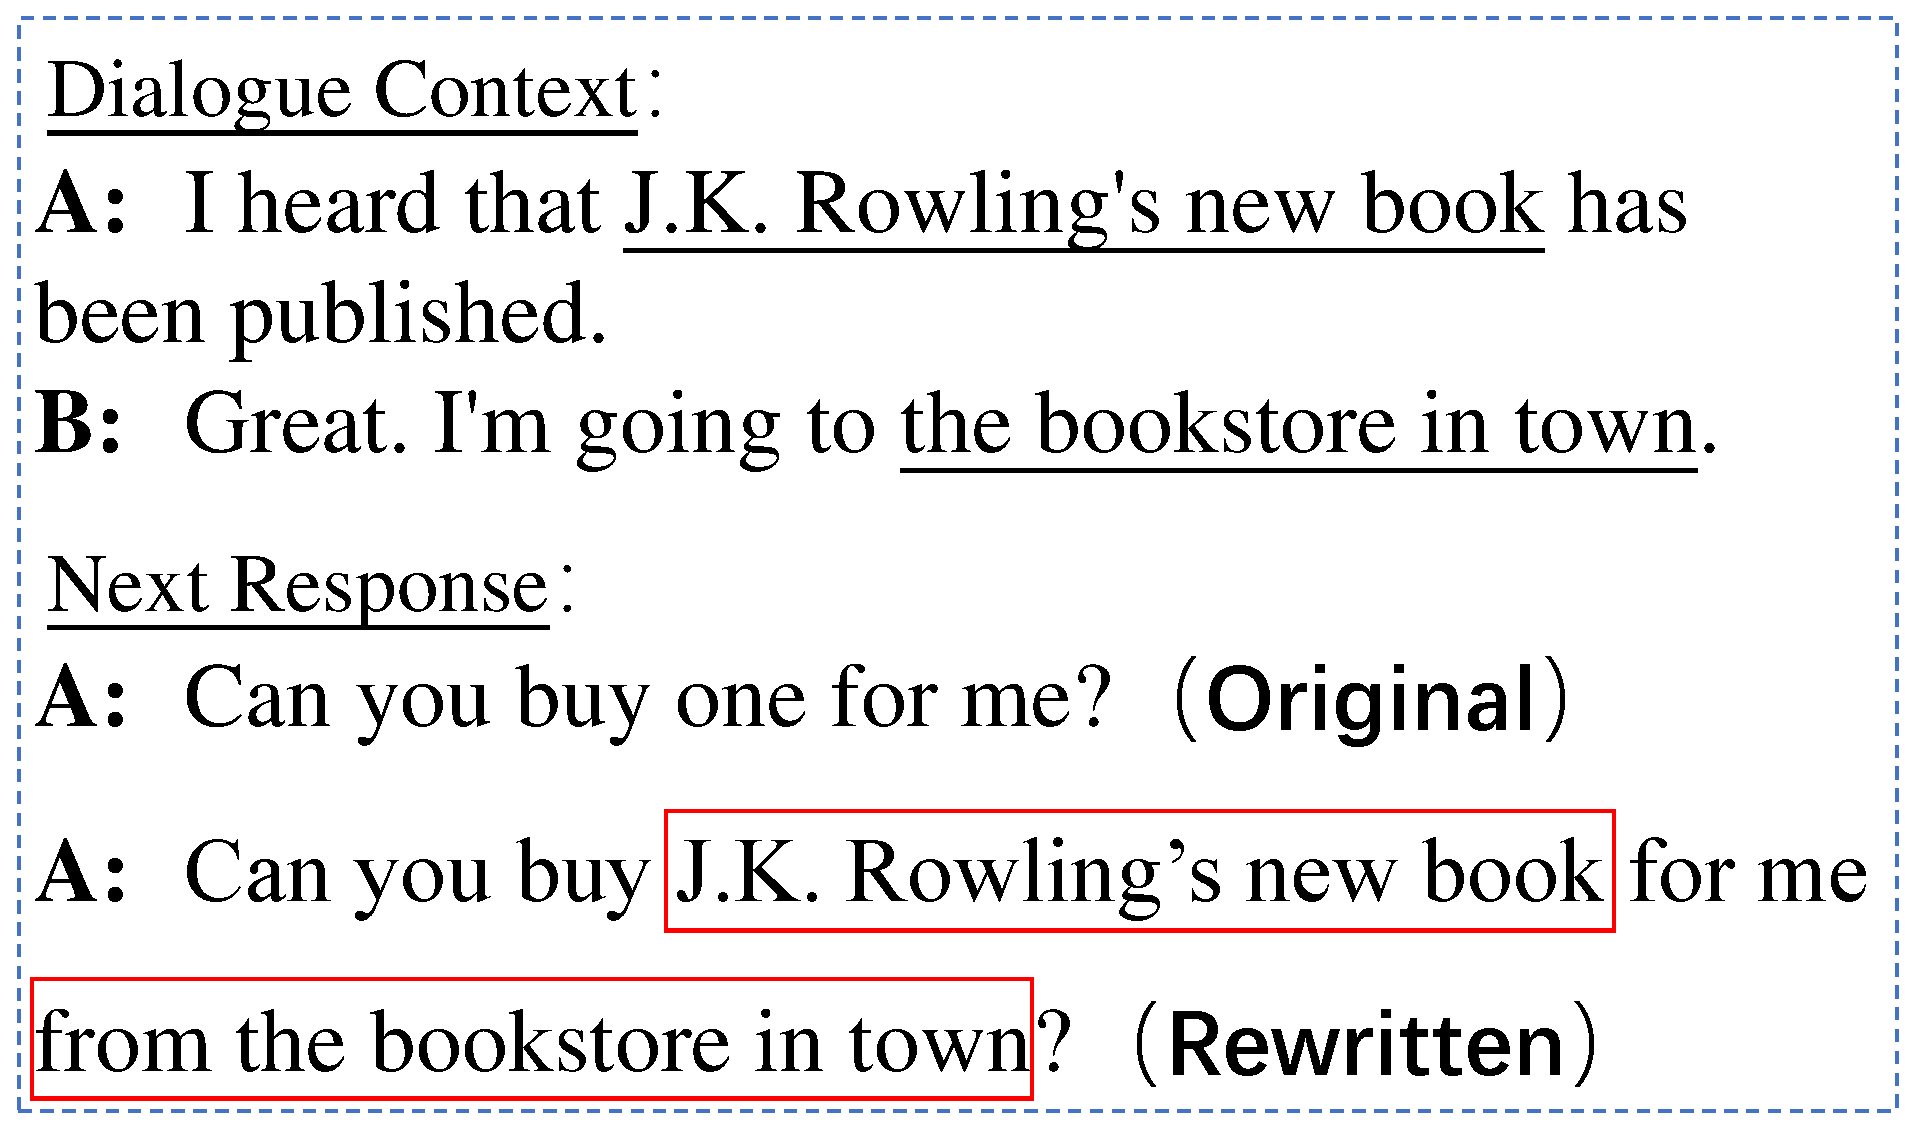
\includegraphics[width=0.8\columnwidth]{rewrite-example.eps}
        \caption{An example of utterance rewriting.}
        \label{fig:rewrite-example}
\end{figure}

%\KZ{The absence of} 
The sources of incompletion of an utterance can be divided into two categories: coreference and ellipsis. 
The task for solving these two kinds of imcompletion is named as Incomplete Utterance Rewriting (IUR). 
As shown in \figref{fig:rewrite-example}, the third utterance of this multi-turn dialogue is incomplete. If this utterance is taken out alone without context, 
%the third party 
we will not be able to 
understand what ``one'' means and where to buy it. The fourth utterance is a rewriting of the third utterance. We can see that ``one'' in the third utterance is replaced by ``J.K. Rowling's new book''. In addition, the place adverbial ``from the book store in town'' is inserted after ``for me''. %These two examples show the coreference and ellipsis respectively within an incomplete utterance.
In the industrial production and online environment, due to the requirements of running time and maintenance cost, the single-turn model is much more 
applicable than the multi-turn models.
If incomplete sentences can be rewritten, 
making it understandable without context, the cost of downstream NLP tasks, such as intention extraction and response generation, will be reduced.

From \figref{fig:rewrite-example}, we can also find that all the words added in the rewriting 
utterance except ``from'' come from context. Inspired by this, many early rewriting works used 
pointer networks \citep{NIPS2015_29921001} or sequence to sequence models with copy 
mechanism \citep{gu-etal-2016-incorporating, see-etal-2017-get} to directly obtain the parts to 
be added from the context. More recently, pre-trained language models such as T5 \citep{2020t5} is used to
%simply 
solve different NLP tasks.
%But when it is directly used to do IUR task, 
However, IUR task is different from other generation tasks 
as the newly added parts usually
only appear in specific locations in the original utterance.
For example, adding modifiers before or after the central word.
On the contrary, 
end-to-end models
tend to generate
flexibly
without preserving the syntactic structure 
of the original utterance.
As a result,we may lose
some important information
%may be lost 
and 
even bring some 
wrong information to the output
after rewriting, which is shown
as follows.

\begin{itemize}
\item Can you buy \textbf{J.K. Rowling's new book}? (Losing original structure)
\item Can you \textbf{publish} new book for me ? (Bringing in wrong information)
\end{itemize}
%outside
%the positions to rewrite. 
%should be 
%\textcolor{green}{(Ruolan: Why?)}
%Preserving means that 
%IUR task is different from other generation tasks
%as the newly added parts usually 
%only appear in specific locations in the original utterance. 
%For example, adding modifiers before or after the central word.
%This particular characteristic
%makes rewriting task different from other generation tasks.
%\KZ{You need to set up the problem of large search space first by saying the previous approaches suffers from
%large search space because ... and this leads to bad... I also think that you haven't sufficiently
%demonstrated the badness of prev approaches. You can give some bad examples..}
%Instead, end-to-end pre-trained models would create something like these without original syntactic structure.
%\begin{itemize}
%\item Can you buy \textbf{J.K. Rowling's new book}? (Losing original structure)
%\item Can you \textbf{publish} new book for me ? (Bringing in wrong information)
%\end{itemize}
%\textcolor{green}{(Ruolan: Do we need some bad examples?)}

Another problem of the end-to-end pre-trained models, which generate the rewritten utterances from scratch,
is that they generally incurrs a large search space and therefore not only imprecise but also
inefficient.
%The rewriting task does not need to generate the whole utterance from scratch, but only needs to 
%modify the original utterance partially. Previous works\textcolor{green}{Ruolan:reference?} 
%have too large search space. The syntactic structure has been modified unnecessarily. 
In order to solve the large search space issue, %introduced by common generation model,
%\KZ{What is the large search space issue? you haven't even mentioned it
%before. It's too sudden to talk about like this. I think the way prev method works has two negative
%effects: 1) the results are no good because the syntactic structure may be changed; 2) the search space
%is larger. You need to discuss these two issues better.} 
%recently, some works have designed models with smaller search space.
%than generative methods. 
\citet{hao-etal-2021-rast} treated utterance rewriting as 
%multi-task
sequence tagging task. For each input word, they predict whether it should be deleted and the span that needs to be replaced with. \citet{liu-etal-2020-incomplete} formulated IUR as a syntactic segmentation task. They predict segmentation operations required on the utterance to be rewritten. However, they still did not take the step of predicting the rewritten positions alone, and did not effectively model the positions of the rewritten part in the sentence structure, which is important in IUR. If the model can learn the syntactic structure information in the sentence used in rewriting, it can predict which part of the sentence should be modified, that is to say, which words need to be replaced and where new words need to be inserted. 
After that, the model only needs to fill in these predicted positions. These two tasks are relatively simple, but they can efficiently use the structure of rewriting sentences.
%this
Our 
paper is based on the above.

In order to effectively utilize the syntactic structure of the sentence to be rewritten, we divide the IUR task into two phases. The first phase is to predict which positions in the utterance need to be rewritten (including coreference and ellipsis). The second phase is to fill in the predicted positions. In the first phase, we use the sequence annotation method to predict the locations of coreference and ellipsis in the utterance. In the second phase, we take the 
utterances with blanks as input
%fine-tune the pre-trained language model, 
and directly predict the words required for the blank position.
By seperating the
original rewriting
task into two relatively simple phases, 
our results show that 
our model performs the best among 
recent state-of-the-art
rewriting models. 
%\KZ{Give an intuition why this might work better.}

Our main contributions are as follows. 
\begin{itemize}
\item A highly extensive two-phase framework for solving incomplete utterance rewriting task is 
proposed, which achieves the best results on multiple public datasets. (\secref{sec:2-step-supervised-method})
\item  An algorithm 
for succinctly and efficiently
generating training data
based on the longest common subsequences (LCS)
algorithm. 
%is designed
%, which can 
%preprocess and automatically label the rewriting dataset, and label the rewritten part 
%according to the sentences before and after rewriting to obtain the training data. 
We generated 
two kinds of data
which 
can be used for 
predicting the positions to be rewritten (the first phase)
%sequence annotation
and filling the blanks (the second phase)
respectively. (\secref{sec:becky-lcs})
%which is our method to predict the positions to be rewritten.
%\KZ{Too long-winded.}
\item  Pre-trained language model is used to fill in the positions to be rewritten in the utterance, 
while adding prompts and spliting utterance according to the number of blanks are used to improve model's performance. (\secref{blanks-filling})
%\item %We demonstrate the improvements in efficiency 
%using direct chat logs between bots.
%\KZ{Maybe this should not be a contribution but part of the conclusion?}
%We show that the chats between bots are impressively informative, 
%even richer than the chats between humans and bots.
%This suggests some possible directions to improve 
%the capabilities of bots in the future.
%(e.g., by having them learn from each other)  (\secref{sec:diversity})
\end{itemize}
